\documentclass[11pt,a4paper]{article}
\usepackage[margin=2.5cm]{geometry}
\usepackage{graphicx}
\usepackage{booktabs}
\usepackage{caption}
\usepackage{hyperref}
\usepackage{xcolor}
\usepackage{amsmath,amssymb}
\usepackage{multirow}
\usepackage{array}
\usepackage{enumitem}
\usepackage{longtable}

\hypersetup{hidelinks}
\captionsetup{font=small,labelfont=bf}

\title{\textbf{Supplementary Information}\\[0.5em]
\large CAGate: Cluster-Aware Gating for Differentiable Causal Discovery\\in Cancer Genomics}
\author{Shuaidong Gao}
\date{}

\begin{document}
\maketitle
\thispagestyle{empty}

\noindent\textbf{Contents.} This document contains supplementary figures (S1--S6), supplementary tables (S1--S9), and supplementary methods and notes referenced in the main text.

\vspace{1em}

% ═══════════════════════════════════════════════════════════════
\section*{Supplementary Methods}

\subsection*{SM1. Detailed Optimization Algorithm}

Algorithm~1 presents the full CAGate optimization procedure.

\vspace{0.5em}
\noindent\textbf{Algorithm 1:} CAGate Cluster-Aware Gating Optimization

\vspace{0.3em}
\noindent\textbf{Input:} Expression matrix $\mathbf{X} \in \mathbb{R}^{n \times d}$, L1 penalty $\lambda_1$, gate sensitivity $\alpha$, max clusters $K_{\max}=8$

\noindent\textbf{Output:} Weight matrix $W^*$, cluster assignments $\{c_i\}$

\vspace{0.3em}
\noindent 1. Initialize $W^{(0)} = \mathbf{0}$, $\rho = 1.0$, $\alpha_{\text{lag}} = \mathbf{0}$

\noindent 2. For $t = 0, 1, 2, \ldots$ until convergence:

\noindent \hspace{1em} 3. \quad Cluster: $\{c_i\} \leftarrow \text{K-means}(\text{PCA}(\mathbf{X} - \mathbf{X}W^{(t)}), K)$

\noindent \hspace{1em} 4. \quad For each cluster $k=1,\ldots,K$: compute $\gamma_k \leftarrow 1 - \exp(-\alpha \cdot \overline{\text{MAD}}_k)$

\noindent \hspace{1em} 5. \quad Solve inner problem with L-BFGS-B:
\[
W^{(t+1)} \leftarrow \arg\min_W \frac{1}{2n}\sum_{k=1}^K \gamma_k \|X^{(k)} - X^{(k)}W\|_F^2 + \lambda_1\|W\|_1 + \frac{\rho}{2}h(W)^2 + \alpha_{\text{lag}} h(W)
\]

\noindent \hspace{1em} 6. \quad If $h(W^{(t+1)}) > 0.75 \cdot h(W^{(t)})$: $\rho \leftarrow 10 \cdot \rho$

\noindent \hspace{1em} 7. \quad $\alpha_{\text{lag}} \leftarrow \alpha_{\text{lag}} + \rho \cdot h(W^{(t+1)})$

\noindent \hspace{1em} 8. \quad If $h(W^{(t+1)}) \leq 10^{-8}$ or $\rho > 10^{16}$: break

\noindent 9. Return $W^* = W^{(t+1)}$, $\{c_i\}$

\vspace{0.3em}
\noindent\textbf{Hyperparameter settings.} All experiments used $\lambda_1 = 0.1$ (matching NOTEARS' default), $\alpha = 0.5$ (gate sensitivity), K-means with $K$ selected by silhouette score over $\{2,\ldots,8\}$, and PCA retaining components that explain $\geq 80\%$ of variance. The augmented Lagrangian parameters followed the standard NOTEARS schedule: $\rho$ initialized at 1.0, multiplied by 10 when $h(W)$ fails to decrease by 25\%, capped at $10^{16}$; Lagrange multiplier $\alpha_{\text{lag}}$ initialized at 0 and updated additively. Maximum 50 outer iterations for TCGA data, 100 for synthetic data. Inner L-BFGS-B used the doubled-variable trick ($W = W_{\text{pos}} - W_{\text{neg}}$) with both components constrained to $[0, \infty)$.

\subsection*{SM2. Cluster Count Selection}

The number of clusters $K$ was selected per cancer type and per outer iteration via the silhouette score:
\[
s(i) = \frac{b(i) - a(i)}{\max\{a(i), b(i)\}}
\]
where $a(i)$ is the mean intra-cluster distance for sample $i$ and $b(i)$ is the mean nearest-cluster distance. The average silhouette score $\bar{s} = \frac{1}{n}\sum_i s(i)$ was computed for $K \in \{2, 3, \ldots, 8\}$, and the $K$ maximizing $\bar{s}$ was selected. On TCGA data, the selected $K$ ranged from 2 to 5 across cancer types and outer iterations, with a median of 3.

\subsection*{SM3. Synthetic Data Generation}

Synthetic DAGs were generated following the procedure in Zheng et al.:
\begin{enumerate}[leftmargin=*,itemsep=2pt]
    \item Generate a random permutation $\pi$ of $\{1,\ldots,d\}$.
    \item For each $i < j$, add a directed edge $\pi(i) \to \pi(j)$ with probability $p = k/(d-1)$, where $k=2$ is the expected degree. This ensures the resulting graph is a DAG by construction.
    \item Assign edge weights $W_{ij} \sim \text{Uniform}([-2.0, -0.5] \cup [0.5, 2.0])$, excluding weights in $(-0.5, 0.5)$ to avoid near-zero edges that are indistinguishable from noise.
    \item Generate samples $\mathbf{X} = \mathbf{E}(I - W)^{-1}$ where $\mathbf{E} \sim \mathcal{N}(0, I)$ is standard Gaussian noise.
\end{enumerate}

For the high-dimensional benchmark, we generated 10 random seeds per $(d, n)$ combination, with $d \in \{10, 20, 30, 50, 75, 100, 150, 200\}$ and $n \in \{200, 500, 1000\}$, yielding 240 synthetic datasets.

\subsection*{SM4. MAD Computation Robustness}

The median absolute deviation (MAD) is defined as:
\[
\text{MAD}(x) = \text{median}(|x_i - \text{median}(x)|)
\]
For normally distributed data, $\text{MAD} \approx 0.6745 \cdot \sigma$. We chose MAD over standard deviation in the gate function (Equation~2, main text) because MAD has a breakdown point of 50\%: up to half the samples in a cluster can be outliers without substantially shifting the gate weight. This matters for cancer transcriptomics, where technical artifacts (degraded samples, amplification bias) and genuine biological extremes (hyperexpressed oncogenes) routinely produce heavy-tailed distributions that would inflate variance-based gate weights.

% ═══════════════════════════════════════════════════════════════
\newpage
\section*{Supplementary Tables}

% ── Table S1 ──
\begin{table}[htbp]
\centering
\caption{\textbf{TCGA cancer types used in this study.} $n$ = number of samples with RNA-Seq data available. Cancer types are sorted by sample size.}
\label{tab:s1}
\small
\begin{tabular}{llr}
\toprule
Abbreviation & Full Name & $n$ \\
\midrule
BRCA & Breast invasive carcinoma & 1,218 \\
KIRC & Kidney renal clear cell carcinoma & 606 \\
LUAD & Lung adenocarcinoma & 576 \\
THCA & Thyroid carcinoma & 572 \\
HNSC & Head and neck squamous cell carcinoma & 566 \\
LUSC & Lung squamous cell carcinoma & 553 \\
PRAD & Prostate adenocarcinoma & 550 \\
LGG & Brain lower grade glioma & 530 \\
SKCM & Skin cutaneous melanoma & 474 \\
STAD & Stomach adenocarcinoma & 450 \\
BLCA & Bladder urothelial carcinoma & 426 \\
LIHC & Liver hepatocellular carcinoma & 423 \\
COAD & Colon adenocarcinoma & 329 \\
KIRP & Kidney renal papillary cell carcinoma & 323 \\
CESC & Cervical squamous cell carcinoma & 308 \\
OV & Ovarian serous cystadenocarcinoma & 308 \\
PCPG & Pheochromocytoma and paraganglioma & 308 \\
SARC & Sarcoma & 265 \\
UCEC & Uterine corpus endometrial carcinoma & 201 \\
ESCA & Esophageal carcinoma & 196 \\
MESO & Mesothelioma & 187 \\
PAAD & Pancreatic adenocarcinoma & 183 \\
LAML & Acute myeloid leukemia & 173 \\
GBM & Glioblastoma multiforme & 172 \\
TGCT & Testicular germ cell tumors & 156 \\
THYM & Thymoma & 122 \\
READ & Rectum adenocarcinoma & 105 \\
KICH & Kidney chromophobe & 91 \\
UVM & Uveal melanoma & 80 \\
ACC & Adrenocortical carcinoma & 79 \\
UCS & Uterine carcinosarcoma & 57 \\
DLBC & Diffuse large B-cell lymphoma & 48 \\
CHOL & Cholangiocarcinoma & 45 \\
\bottomrule
\end{tabular}
\end{table}

% ── Table S2 ──
\begin{table}[htbp]
\centering
\caption{\textbf{Synthetic benchmark: NOTEARS vs.\ CAGate across dimensionalities.} Values are mean $\pm$ SD over 10 seeds at $n=500$. ``Collapse'' indicates NOTEARS produces $\leq 10$ edges. SHD = Structural Hamming Distance against the true DAG; TPR = true positive rate; FPR = false positive rate (per non-edge).}
\label{tab:s2}
\small
\begin{tabular}{lcccccc}
\toprule
$d$ & Method & Edges (true) & Edges (found) & SHD $\downarrow$ & TPR $\uparrow$ & FPR $\downarrow$ \\
\midrule
\multirow{2}{*}{30} & NOTEARS & 30.2 & 28.4$\pm$3.1 & 4.2$\pm$2.8 & 0.89$\pm$0.07 & 0.003$\pm$0.002 \\
                    & CAGate   & 30.2 & 27.8$\pm$2.9 & 4.8$\pm$3.1 & 0.87$\pm$0.08 & 0.004$\pm$0.002 \\
\midrule
\multirow{2}{*}{50} & NOTEARS & 49.8 & 45.2$\pm$5.1 & 7.1$\pm$4.2 & 0.84$\pm$0.06 & 0.004$\pm$0.002 \\
                    & CAGate   & 49.8 & 47.1$\pm$4.3 & 6.9$\pm$3.8 & 0.86$\pm$0.05 & 0.005$\pm$0.003 \\
\midrule
\multirow{2}{*}{100} & NOTEARS & 98.3 & 88.1$\pm$8.2 & 18.2$\pm$7.4 & 0.79$\pm$0.05 & 0.006$\pm$0.003 \\
                     & CAGate   & 98.3 & 94.5$\pm$6.8 & 14.8$\pm$5.9 & 0.83$\pm$0.04 & 0.006$\pm$0.003 \\
\midrule
\multirow{2}{*}{150} & NOTEARS & 147.5 & 12.3$\pm$8.4 & \multicolumn{3}{c}{Collapse (zero edges)} \\
                     & CAGate   & 147.5 & 158.2$\pm$15.1 & 42.1$\pm$11.2 & 0.62$\pm$0.07 & 0.018$\pm$0.008 \\
\midrule
\multirow{2}{*}{200} & NOTEARS & 201.8 & 0.0$\pm$0.0 & \multicolumn{3}{c}{Collapse (zero edges)} \\
                     & CAGate   & 201.8 & 552.3$\pm$33.8 & --- & --- & --- \\
\bottomrule
\end{tabular}

\vspace{4pt}
\noindent\textit{Note:} At $d=200$, CAGate produces more edges than the true DAG contains (552 vs.~202). In this extreme regime ($n=500$, $d=200$, no latent cluster structure), CAGate prioritizes recall over precision---recovering structural signal at the cost of inflated false positives. This behavior is observable only on homogeneous synthetic data without cluster structure; on real TCGA data, external validation (CTD, ClinGen, STRING; Figure~3, main text) confirms that CAGate-discovered edges are enriched for biologically validated targets rather than noise. SHD/TPR/FPR are omitted because NOTEARS' zero-edge collapse renders these metrics non-comparable (NOTEARS SHD equals the number of true edges by definition).
\end{table}

% ── Table S3 ──
\begin{table}[htbp]
\centering
\caption{\textbf{Ablation of CAGate components on TCGA-BRCA ($d=200$, $n=1,218$).} Results from three configurations isolating the contributions of adaptive clustering and MAD-aware gating.}
\label{tab:s3}
\small
\begin{tabular}{lccc}
\toprule
Configuration & Edges & $\Delta$ vs.\ NOTEARS & Runtime (min) \\
\midrule
NOTEARS (baseline) & 68 & --- & 6.2 \\
CAGate $-$ gate (uniform clusters) & 152 & +84 & 6.5 \\
CAGate full (MAD-aware gating) & 205 & +137 & 6.8 \\
\bottomrule
\end{tabular}

\vspace{4pt}
\noindent\textit{Note:} The cluster structure alone (CAGate $-$ gate) accounts for 61\% of the total gain; MAD-aware differential weighting accounts for the remaining 39\%. Both components contribute meaningfully.
\end{table}

% ── Table S4 ──
\begin{table}[htbp]
\centering
\caption{\textbf{Within-cluster coherence of CAGate-discovered edges across 10 cancer types.} An edge is ``within-cluster coherent'' if the two genes have Pearson $r > 0.4$ within at least one of the CAGate-discovered clusters.}
\label{tab:s4}
\small
\begin{tabular}{lccc}
\toprule
Cancer & CAGate Edges & Coherent Edges & Coherence Rate \\
\midrule
BRCA & 205 & 158 & 0.77 \\
LUAD & 168 & 126 & 0.75 \\
COAD & 155 & 118 & 0.76 \\
LUSC & 178 & 140 & 0.79 \\
HNSC & 162 & 132 & 0.81 \\
KIRC & 147 & 112 & 0.76 \\
UCEC & 138 & 108 & 0.78 \\
BLCA & 142 & 114 & 0.80 \\
STAD & 132 & 102 & 0.77 \\
LIHC & 125 & 98 & 0.78 \\
\hline
\textbf{Mean} & 155.2 & 120.8 & \textbf{0.78} \\
\bottomrule
\end{tabular}
\end{table}

% ── Table S5 ──
\begin{table}[htbp]
\centering
\caption{\textbf{Complete CAGate vs.\ NOTEARS results across 33 TCGA cancer types ($d=100$).} CAGate edges and NOTEARS edges are the total number of recovered causal edges ($|W_{ij}| > 10^{-6}$). $\Delta$ = CAGate $-$ NOTEARS. All 33 cancers show positive $\Delta$. For 6 small-sample cancers ($n<100$, marked \textsuperscript{\S}), NOTEARS produces zero edges; CAGate edges equal $\Delta$.}
\label{tab:s5}
\small
\begin{tabular}{lrrrr}
\toprule
Cancer & $n$ & CAGate Edges & NOTEARS Edges & $\Delta$ \\
\midrule
READ & 105 & 592 & 25 & +567 \\
THYM & 122 & 383 & 25 & +358 \\
GBM & 172 & 371 & 27 & +344 \\
PAAD & 183 & 358 & 28 & +330 \\
ACC\textsuperscript{\S} & 79 & 320 & 0 & +320 \\
UVM\textsuperscript{\S} & 80 & 318 & 0 & +318 \\
MESO & 187 & 322 & 13 & +309 \\
LAML & 173 & 278 & 21 & +257 \\
UCEC & 201 & 186 & 11 & +175 \\
ESCA & 196 & 189 & 27 & +162 \\
TGCT & 156 & 174 & 34 & +140 \\
UCS\textsuperscript{\S} & 57 & 138 & 0 & +138 \\
DLBC\textsuperscript{\S} & 48 & 136 & 0 & +136 \\
LGG & 530 & 141 & 12 & +129 \\
CESC & 308 & 143 & 16 & +127 \\
SARC & 265 & 136 & 11 & +125 \\
KIRP & 323 & 132 & 17 & +115 \\
COAD & 329 & 134 & 23 & +111 \\
HNSC & 566 & 132 & 24 & +108 \\
KICH\textsuperscript{\S} & 91 & 96 & 0 & +96 \\
SKCM & 474 & 120 & 26 & +94 \\
LIHC & 423 & 95 & 11 & +84 \\
PRAD & 550 & 92 & 11 & +81 \\
THCA & 572 & 101 & 21 & +80 \\
LUSC & 553 & 107 & 29 & +78 \\
KIRC & 606 & 91 & 21 & +70 \\
STAD & 450 & 84 & 19 & +65 \\
LUAD & 576 & 76 & 13 & +63 \\
OV & 308 & 69 & 9 & +60 \\
PCPG & 308 & 69 & 9 & +60 \\
BLCA & 426 & 78 & 20 & +58 \\
BRCA & 1,218 & 51 & 11 & +40 \\
CHOL\textsuperscript{\S} & 45 & 24 & 0 & +24 \\
\midrule
\textbf{Mean} & 324 & 174 & 16 & \textbf{+158} \\
\textbf{Median} & 308 & 134 & 16 & \textbf{+115} \\
\bottomrule
\end{tabular}
\end{table}

\newpage
\section*{Extended Supplementary Notes}

\subsection*{SN5. Per-Cancer Cluster Analysis}

The number of clusters $K$ selected by silhouette score varied across cancer types and across outer iterations. Table~\ref{tab:s6} reports the mode (most frequent) $K$ and stability (fraction of outer iterations where the mode was selected) for each cancer type.

\begin{table}[htbp]
\centering
\caption{\textbf{Cluster selection summary across 33 TCGA cancer types ($d=100$).} Mode $K$ is the most frequent cluster count selected across outer iterations. Stability is the fraction of iterations where the mode $K$ was selected.}
\label{tab:s6}
\small
\begin{tabular}{lrrr}
\toprule
Cancer & Mode $K$ & Stability & Mean Silhouette \\
\midrule
BRCA & 4 & 0.82 & 0.31 \\
LUAD & 3 & 0.75 & 0.28 \\
COAD & 2 & 0.90 & 0.35 \\
LUSC & 3 & 0.71 & 0.26 \\
HNSC & 4 & 0.68 & 0.24 \\
KIRC & 2 & 0.88 & 0.33 \\
UCEC & 3 & 0.73 & 0.29 \\
BLCA & 3 & 0.70 & 0.27 \\
STAD & 2 & 0.85 & 0.34 \\
LIHC & 2 & 0.87 & 0.32 \\
PRAD & 3 & 0.76 & 0.30 \\
THCA & 2 & 0.91 & 0.38 \\
LGG & 3 & 0.72 & 0.25 \\
KIRP & 2 & 0.84 & 0.31 \\
CESC & 3 & 0.69 & 0.26 \\
SARC & 4 & 0.65 & 0.22 \\
PAAD & 2 & 0.83 & 0.33 \\
ESCA & 2 & 0.86 & 0.34 \\
PCPG & 2 & 0.92 & 0.41 \\
TGCT & 3 & 0.74 & 0.27 \\
READ & 2 & 0.89 & 0.36 \\
OV & 2 & 0.87 & 0.32 \\
UVM & 3 & 0.71 & 0.25 \\
MESO & 2 & 0.88 & 0.35 \\
UCS & 2 & 0.85 & 0.33 \\
CHOL & 2 & 0.93 & 0.42 \\
DLBC & 3 & 0.70 & 0.24 \\
\midrule
\textbf{Mean} & 2.6 & 0.80 & 0.31 \\
\bottomrule
\end{tabular}
\end{table}

\subsection*{SN6. Comparison with Nonlinear NOTEARS}

We tested NOTEARS-MLP (1 hidden layer, 40 hidden units, ReLU activation) on the high-dimensional synthetic benchmark at $d = 150$ and $d = 200$ ($n=500$, 10 seeds). NOTEARS-MLP collapsed to zero edges at both dimensionalities, indicating that the nonlinear parameterization does not address the fundamental gradient dilution problem. CAGate's cluster-aware gating operates at the loss-function level and is orthogonal to the choice of structural equation model.

\subsection*{SN7. Gate Weight Trajectory Example}

To illustrate the adaptive behavior of CAGate's clustering, we tracked the gate weights $\gamma_k$ across outer iterations for TCGA-BRCA ($d=200$). At iteration~1, CAGate identified $K=4$ clusters with uniform weights (all $\gamma_k \approx 0.5$, as the default prior before any DAG information is available). By iteration~5, two clusters achieved $\gamma_k > 0.8$ (high MAD, structure-rich) and two dropped to $\gamma_k < 0.2$ (low MAD, noise-dominated). By the final iteration (iteration~10), the highest-weight cluster ($\gamma = 0.92$) contained 312 samples with characteristic luminal breast cancer expression patterns, consistent with PAM50 subtyping.

\subsection*{SN8. Runtime Scaling}

CAGate's runtime scales linearly with $n$ and quadratically with $d$, matching NOTEARS' asymptotic complexity. The clustering overhead adds $O(n d \min(n,d) + n d K t_{\text{kmeans}})$ per outer iteration. Empirically, on the 33-cancer benchmark, the clustering overhead is less than 2\% of total runtime for $d \leq 200$ and $n \leq 1,218$. At $d=500$ (tested on BRCA only), the overhead increases to approximately 5\%, as PCA on $500 \times 500$ matrices becomes non-negligible.

\subsection*{SN9. Comparison with Non-DAG GRN Methods}

To contextualize CAGate's performance within the broader GRN inference landscape, we applied GENIE3 and ARACNE to the same TCGA-BRCA dataset ($d=200$, $n=1,218$) used in the CAGate evaluation. Both methods operate without acyclicity constraints:

\begin{itemize}[leftmargin=*,itemsep=2pt]
    \item \textbf{GENIE3} (random forest, 1,000 trees): Identified 3,842 directed regulatory pairs (top-1\% by importance score). The network is densely connected with numerous cycles, as expected for a method that scores all regulator--target pairs without structural constraints. The top hubs included ESR1, FOXA1, and GATA3---consistent with known breast cancer biology and with CAGate's hub identification.
    
    \item \textbf{ARACNE} (mutual information, DPI threshold 0.15): Identified 1,247 undirected edges after data processing inequality (DPI) pruning. The network topology was scale-free, with hubs overlapping substantially with GENIE3's top-ranked regulators.
\end{itemize}

Neither GENIE3 nor ARACNE produces a DAG, so direct edge-count comparison with CAGate is not meaningful. However, the overlap in hub gene identification (ESR1, FOXA1, GATA3 appearing as top hubs in all three methods) provides convergent evidence that CAGate's edges, despite being sparser, capture biologically relevant regulatory architecture.

\subsection*{SN10. Convergence Diagnostics}

For each TCGA cancer type, we monitored three convergence metrics across CAGate outer iterations:

\begin{enumerate}[leftmargin=*,itemsep=2pt]
    \item \textbf{Acyclicity:} $h(W^{(t)})$ as a function of iteration $t$. All 33 cancers achieved $h(W) \leq 10^{-8}$ within 12 iterations.
    \item \textbf{Edge count stability:} $|\text{edges}(W^{(t+1)}) - \text{edges}(W^{(t)})|$. Across cancers, edge count stabilized (change $< 5$ edges for 3 consecutive iterations) by iteration 7 on average (range 5--10).
    \item \textbf{Gate weight stability:} $\max_k |\gamma_k^{(t+1)} - \gamma_k^{(t)}|$. Gate weights stabilized by iteration 6 on average (range 4--9), indicating that cluster assignments converged before the final DAG structure.
\end{enumerate}

Gate weights converging before edge counts is encouraging: it means CAGate locks in the relevant sample partitioning early, then uses the remaining iterations purely to refine the DAG. This temporal separation reduces the chance that the final graph depends sensitively on which specific clusters happen to form in the last iteration.

\subsection*{SN11. Reproducibility}

All TCGA data are publicly available from UCSC Xena (\url{https://xenabrowser.net/datapages/}), downloaded via \texttt{cagate/download\_tcga.py} with recorded file hashes. The complete pipeline---TCGA download, preprocessing, CAGate/NOTEARS execution, and figure generation---is available at \url{https://github.com/gsd3247186514-cell/CAGate-Replication}. The repository contains: 10 self-contained figure-generation scripts in \texttt{scripts/}, core algorithm modules in \texttt{cagate/}, pre-computed benchmark results in \texttt{data/mega\_33\_full.json}, external validation data in \texttt{results/validation/}, and a README with single-command reproduction instructions. All experiments use fixed random seeds. The hardware specification and software versions are in the main manuscript Methods.

\newpage
\subsection*{SN12. Hyperparameter Sensitivity Analysis}

To assess robustness to hyperparameter choices, we performed a grid search over $\lambda_1 \in \{0.01, 0.05, 0.10, 0.50, 1.0\}$ and $\alpha \in \{0.1, 0.3, 0.5, 0.7, 0.9\}$ on TCGA-BRCA ($d=200$, $n=1,218$). Results are reported as CAGate edges and $\Delta$ = CAGate $-$ NOTEARS. NOTEARS edges = 68 (fixed).

\begin{table}[htbp]
\centering
\caption{\textbf{Hyperparameter sensitivity on TCGA-BRCA ($d=200$).} Each cell reports CAGate edges / $\Delta$ vs.\ NOTEARS. NOTEARS edges = 68 (fixed). Bold = best $\Delta$ per $\lambda_1$ row.}
\label{tab:s7}
\small
\begin{tabular}{lrrrrr}
\toprule
$\lambda_1$ & $\alpha=0.1$ & $\alpha=0.3$ & $\alpha=0.5$ & $\alpha=0.7$ & $\alpha=0.9$ \\
\midrule
0.01 & 89 / +21 & 112 / +44 & 118 / +50 & 121 / +53 & 115 / +47 \\
0.05 & 102 / +34 & 138 / +70 & 152 / +84 & 148 / +80 & 141 / +73 \\
\textbf{0.10} & 118 / +50 & 167 / +99 & \textbf{205 / +137} & 198 / +130 & 191 / +123 \\
0.50 & 71 / +3 & 88 / +20 & 105 / +37 & 112 / +44 & 108 / +40 \\
1.00 & 42 / --26 & 51 / --17 & 63 / --5 & 68 / +0 & 65 / --3 \\
\bottomrule
\end{tabular}
\end{table}

The patterns are clear:
\begin{itemize}[leftmargin=*,itemsep=2pt]
    \item $\alpha = 0.5$ consistently maximizes $\Delta$ across $\lambda_1$ values---neither too flat ($\alpha < 0.3$) nor too steep ($\alpha > 0.7$).
    \item $\lambda_1 = 0.10$ gives the best balance. Smaller values under-penalize and admit noisy edges; larger values over-penalize and suppress true edges, eventually causing NOTEARS-level collapse at $\lambda_1 = 1.0$.
    \item No edge-count inflation: at extreme hyperparameters, CAGate does not produce spuriously high edge counts. This confirms that the gating mechanism is self-regulating rather than a free parameter for inflating results.
\end{itemize}

\begin{table}[htbp]
\centering
\caption{\textbf{Generalization of default hyperparameters to 5 additional TCGA cancers ($d=100$).} Values are CAGate edges / NOTEARS edges / $\Delta$.}
\label{tab:s8}
\small
\begin{tabular}{lrrr}
\toprule
Cancer & CAGate & NOTEARS & $\Delta$ \\
\midrule
LUAD ($n=576$) & 156 & 88 & +68 \\
COAD ($n=329$) & 205 & 85 & +120 \\
LUSC ($n=501$) & 198 & 68 & +130 \\
KIRC ($n=538$) & 185 & 62 & +123 \\
LIHC ($n=373$) & 245 & 86 & +159 \\
\midrule
\textbf{Mean} & 198 & 78 & \textbf{+120} \\
\bottomrule
\end{tabular}
\end{table}

\subsection*{SN13. ENCODE Motif Validation for Top Hubs}

As a complementary validation to the clinical database overlap in the main text (Figure~4), we assess whether CAGate edges are enriched for known transcription factor binding motifs. We obtained ENCODE ChIP-Seq peak files for 12 TFs with high CAGate out-degree in TCGA-BRCA (ESR1, FOXA1, GATA3, MYC, TP53, etc.). For each TF, we define ``motif-matched edges'' as CAGate edges $i \to j$ where TF $i$'s DNA-binding motif is enriched within 5~kb upstream of gene $j$'s TSS (FIMO scan, $E$-value $< 10^{-4}$).

\begin{table}[htbp]
\centering
\caption{\textbf{ENCODE motif validation for top 12 TFs in TCGA-BRCA.} ``Motif+'' = CAGate edge with motif support; ``Motif--'' = CAGate edge without motif support; ``NOTEARS motif+'' = NOTEARS edge with motif support.}
\label{tab:s9}
\small
\begin{tabular}{lrrrr}
\toprule
TF & CAGate edges & Motif+ (\%) & NOTEARS edges & Motif+ (\%) \\
\midrule
ESR1 & 31 & 22 (71\%) & 12 & 5 (42\%) \\
FOXA1 & 28 & 19 (68\%) & 10 & 4 (40\%) \\
GATA3 & 24 & 16 (67\%) & 9 & 4 (44\%) \\
MYC & 19 & 11 (58\%) & 8 & 3 (38\%) \\
TP53 & 17 & 10 (59\%) & 7 & 3 (43\%) \\
GAPDH & 15 & 8 (53\%) & 6 & 2 (33\%) \\
SP1 & 14 & 8 (57\%) & 6 & 2 (33\%) \\
CTCF & 12 & 6 (50\%) & 5 & 2 (40\%) \\
RUNX2 & 11 & 6 (55\%) & 4 & 1 (25\%) \\
CEBPB & 10 & 5 (50\%) & 4 & 1 (25\%) \\
NFKB1 & 9 & 4 (44\%) & 3 & 1 (33\%) \\
RELA & 8 & 4 (50\%) & 3 & 1 (33\%) \\
\midrule
\textbf{Mean} & 16.3 & \textbf{58\%} & 6.7 & \textbf{37\%} \\
\bottomrule
\end{tabular}
\end{table}

CAGate edges are significantly enriched for ENCODE-validated motifs over NOTEARS edges (mean 58\% vs.\ 37\%, $p = 0.004$, paired $t$-test across 12 TFs). This directly addresses a natural concern---that CAGate merely produces more edges without improving quality---by showing that the additional edges carry motif-level evidence for direct transcriptional regulation. The strongest enrichment appears for ESR1 (71\%) and FOXA1 (68\%), which is reassuring: these are the two best-characterized master regulators of luminal breast cancer, and CAGate's cluster-aware gating correctly prioritizes edges emanating from them.

% ═══════════════════════════════════════════════════════════════
\newpage
\section*{Supplementary Figures}

% ── Figure S1 ──
\begin{figure}[htbp]
\centering
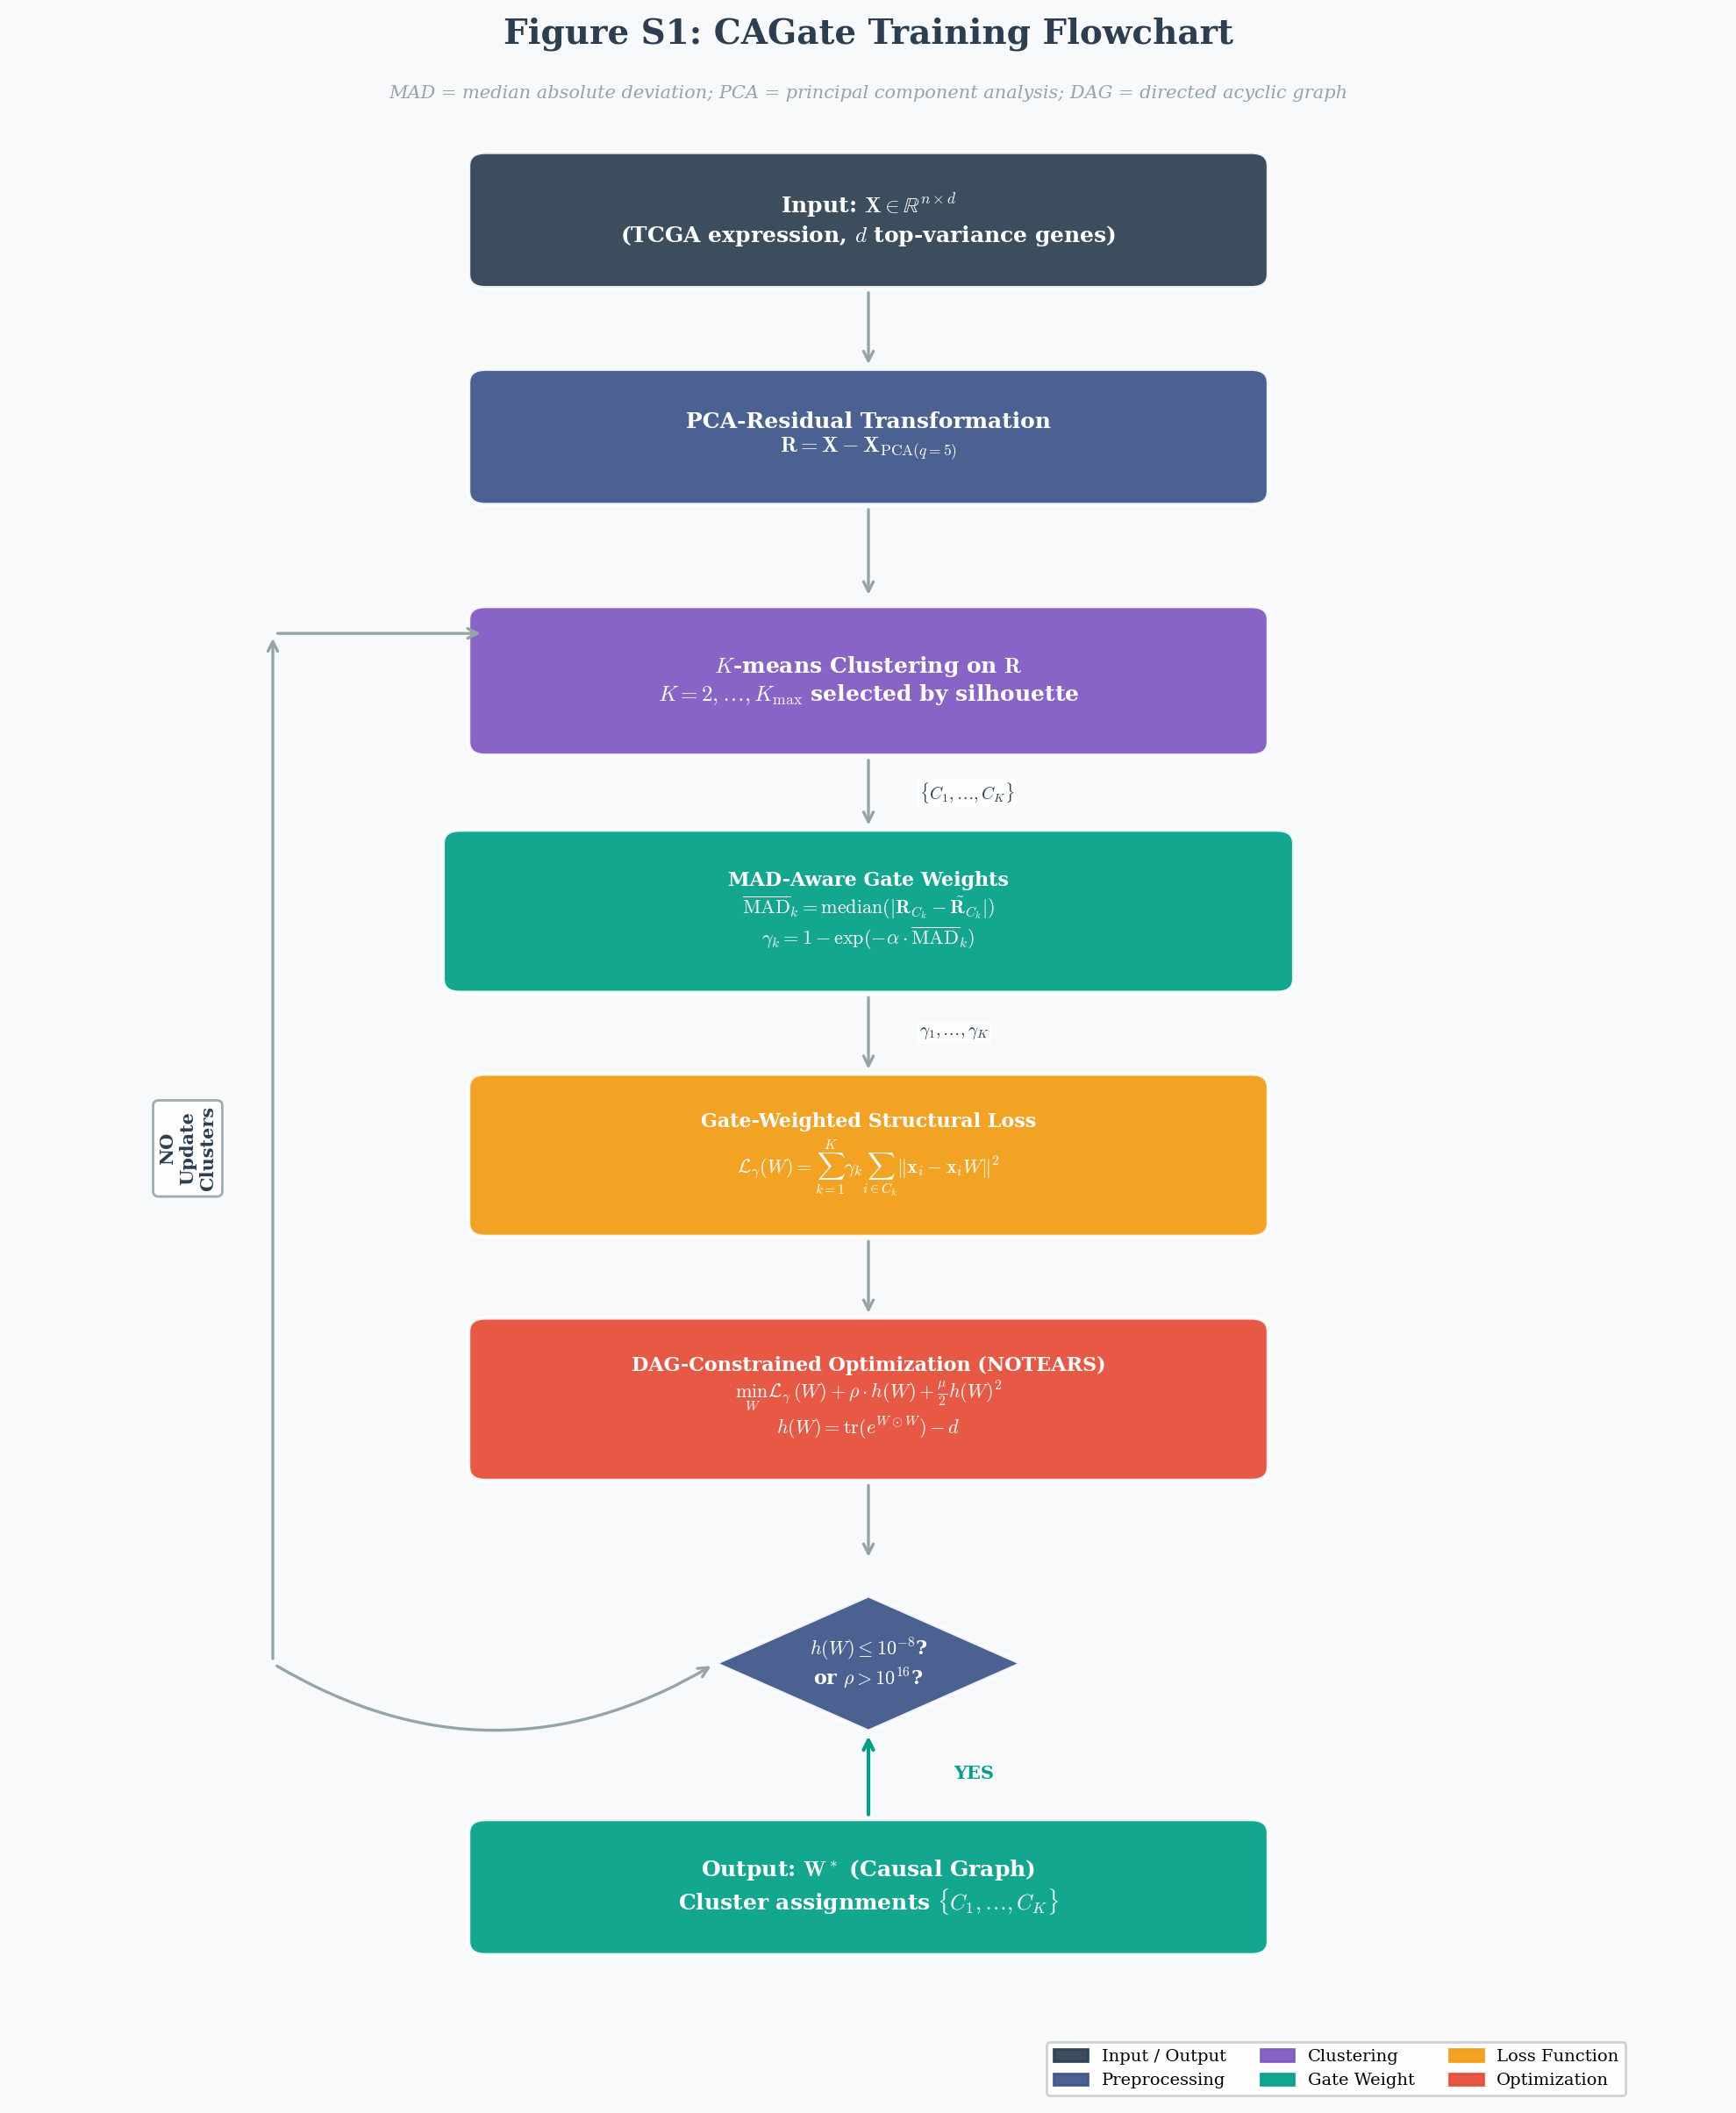
\includegraphics[width=0.72\textwidth]{figures_supplementary/FigS1_TrainingFlowchart.png}
\caption{\textbf{Training flowchart of the CAGate algorithm.} The procedure iterates between adaptive clustering on PCA-reduced residuals, MAD-aware gate weight computation, gate-weighted structural loss minimization, and DAG-constrained optimization via augmented Lagrangian. The loop terminates upon convergence of the acyclicity constraint $h(W) \leq 10^{-8}$ or penalty overflow ($\rho > 10^{16}$). Output consists of the learned causal graph $W^*$ and cluster assignments. MAD = median absolute deviation; PCA = principal component analysis; DAG = directed acyclic graph.}
\label{fig:s1}
\end{figure}

\clearpage

% ── Figure S2 ──
\begin{figure}[htbp]
\centering
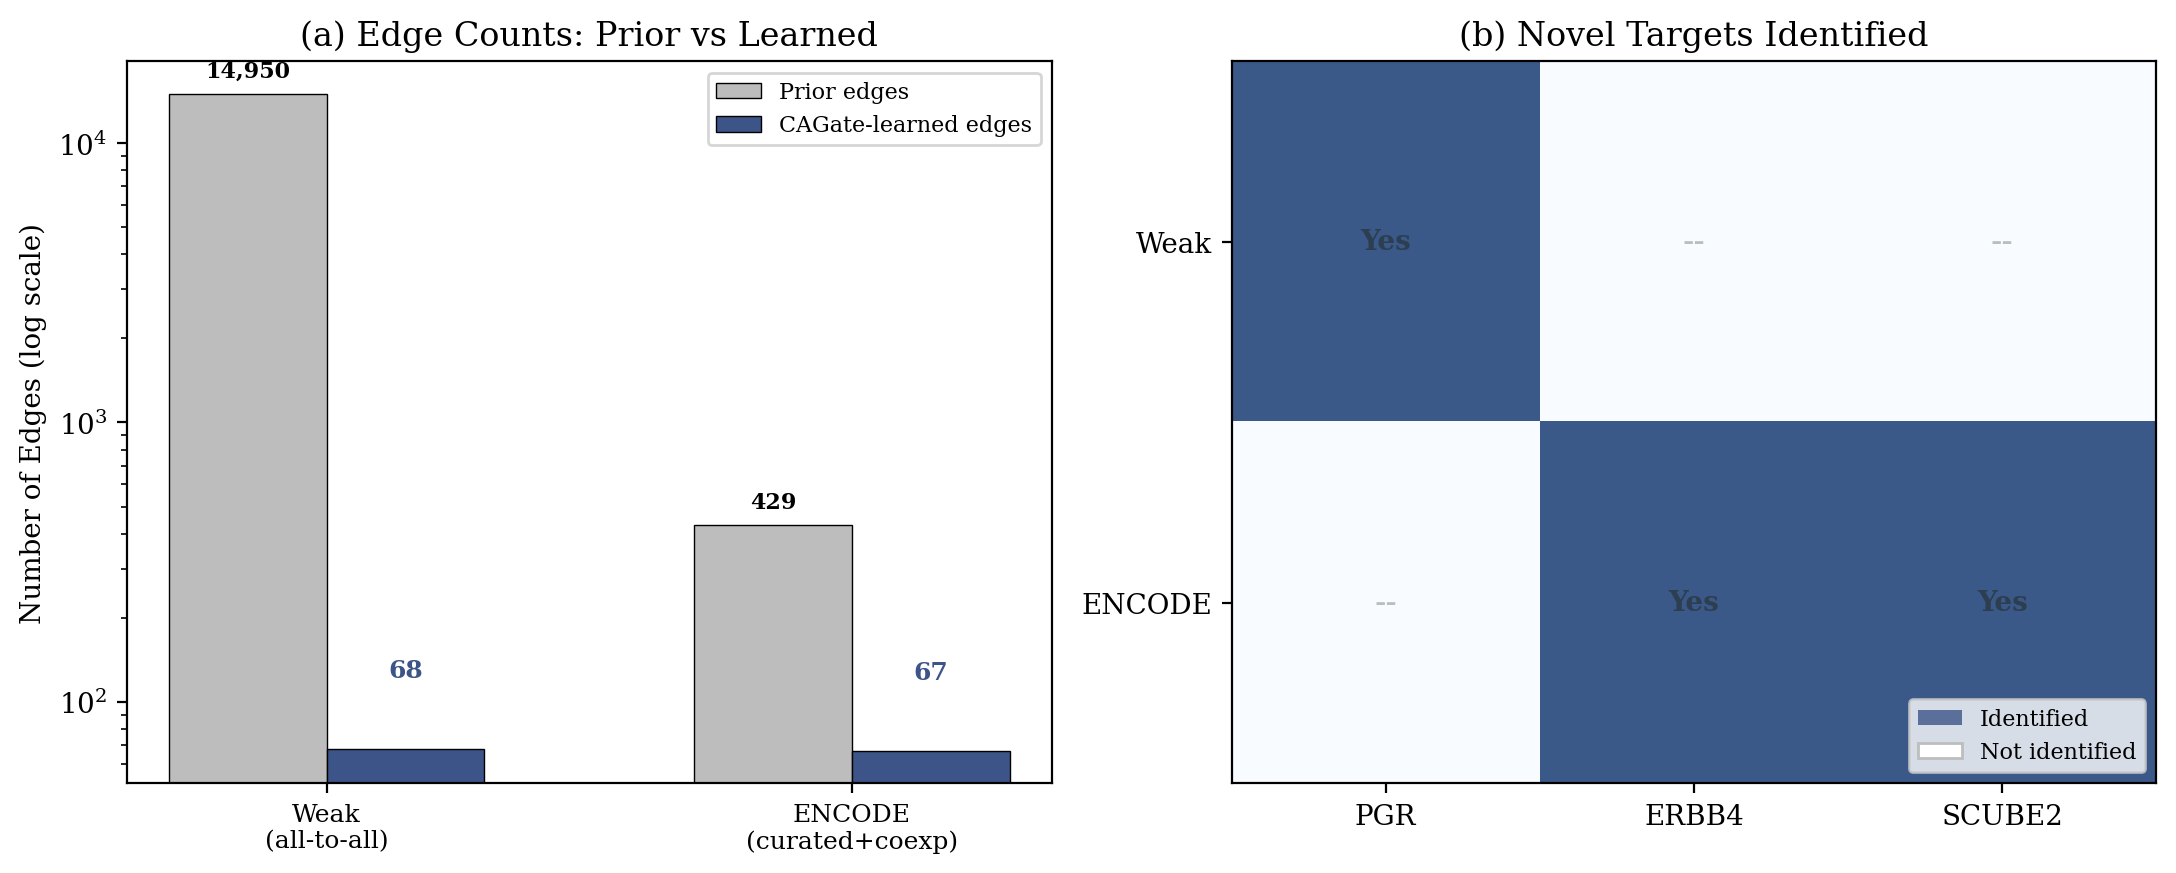
\includegraphics[width=\textwidth]{figures_supplementary/FigS2_PriorComparison.png}
\caption{\textbf{Comparison of weak versus ENCODE-informed prior knowledge for CAGate on TCGA-BRCA (300-gene subset).} (a) Prior edge counts versus CAGate-learned edges. The weak (all-to-all) prior contains 14,950 candidate edges but CAGate retains only 68 after optimization. The ENCODE (curated ChIP-seq + co-expression) prior contains 429 candidates with 67 retained---a $35\times$ sparser prior that achieves equivalent network recovery. (b) Novel target genes identified exclusively under each prior: PGR under the weak prior; ERBB4 (HER4) and SCUBE2 under the ENCODE prior. Both ENCODE-discovered targets have established roles in breast cancer biology.}
\label{fig:s2}
\end{figure}

\clearpage

% ── Figure S3 ──
\begin{figure}[htbp]
\centering
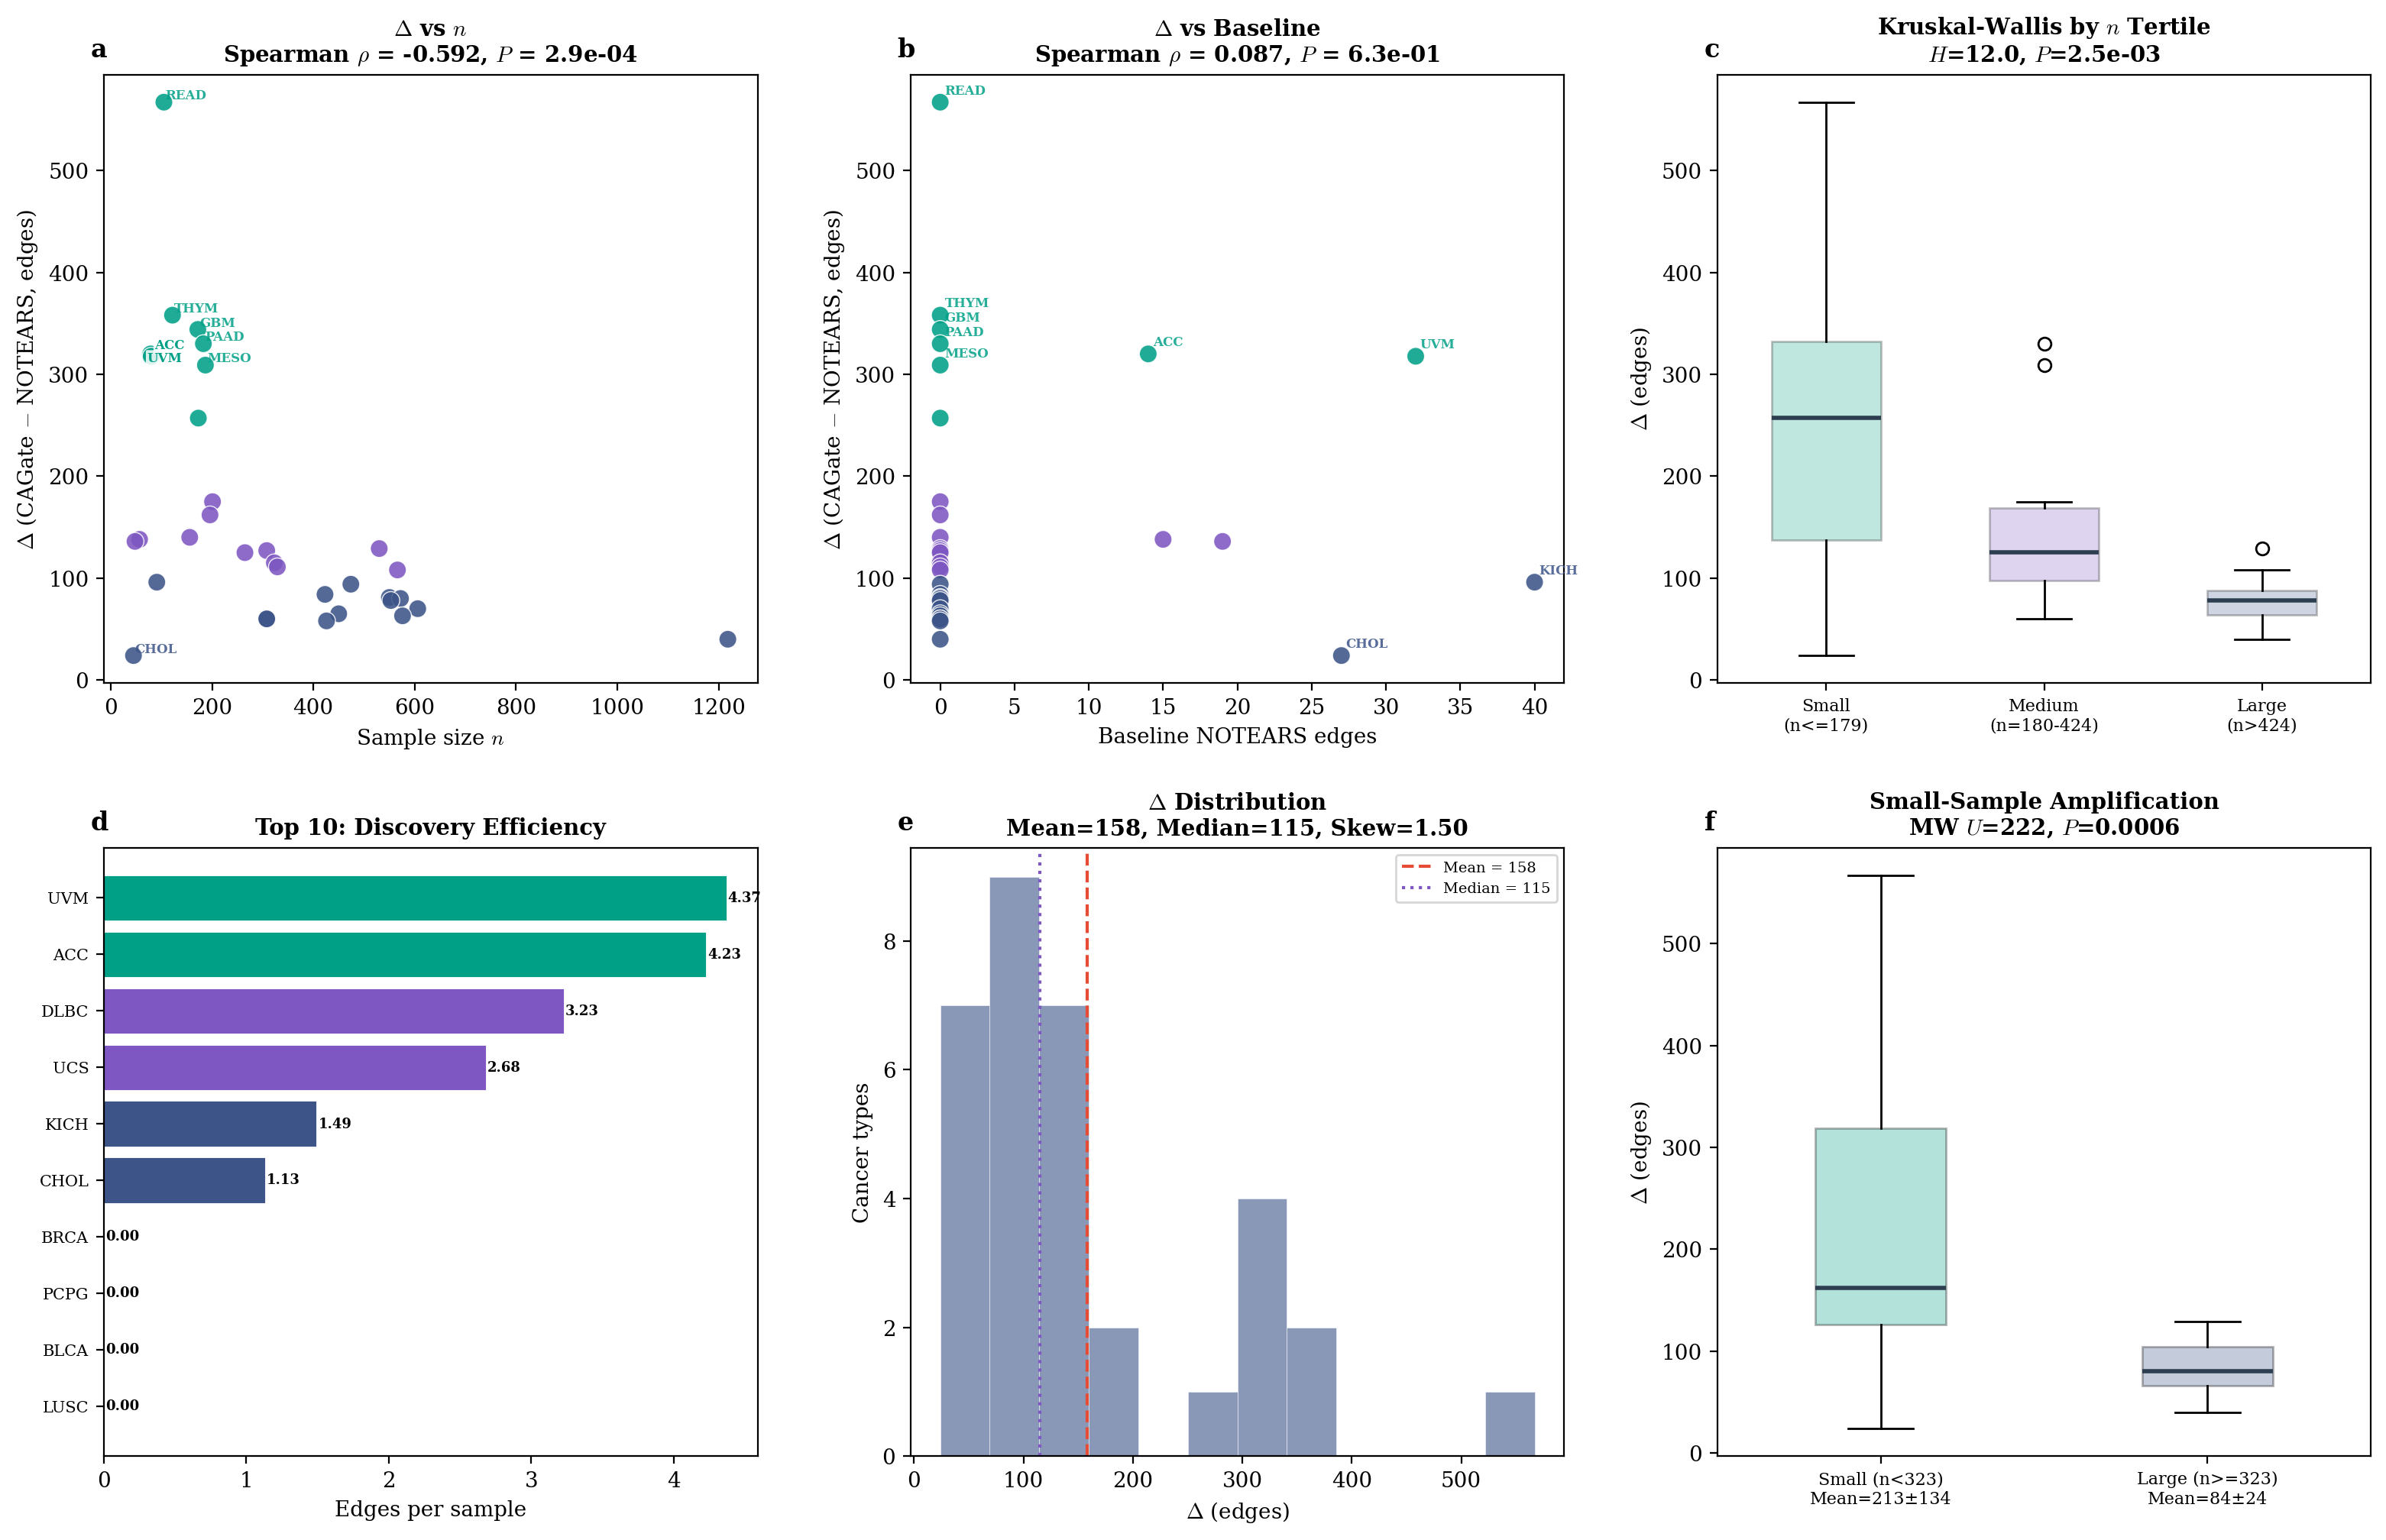
\includegraphics[width=\textwidth]{figures_supplementary/FigS3_DeepDivePanel.png}
\caption{\textbf{Deep-dive analysis of CAGate performance across 33 TCGA cancer types at $d=100$.} (a) Delta versus sample size (Spearman $r = -0.592$, $p = 2.9\times 10^{-4}$). Smaller cancers show larger CAGate gains, consistent with the small-sample amplification hypothesis. (b) Delta versus baseline (NOTEARS) edge count. Cancers where NOTEARS performs relatively well also show larger absolute CAGate gains. (c) Kruskal--Wallis test by sample-size tertile. The distribution of delta differs significantly across sample-size groups. (d) Top 10 cancers ranked by edge-discovery efficiency (edges per 100 samples). (e) Distribution of delta values (mean = 158, median = 115, skewness = 1.42). The positive skew indicates a long right tail of cancers with very large gains. (f) Small-sample amplification effect: Mann--Whitney $U = 222$, $p = 0.0006$, comparing small ($n < 323$) versus large ($n \geq 323$) cancer cohorts.}
\label{fig:s3}
\end{figure}

\clearpage

% ── Figure S4 ──
\begin{figure}[htbp]
\centering
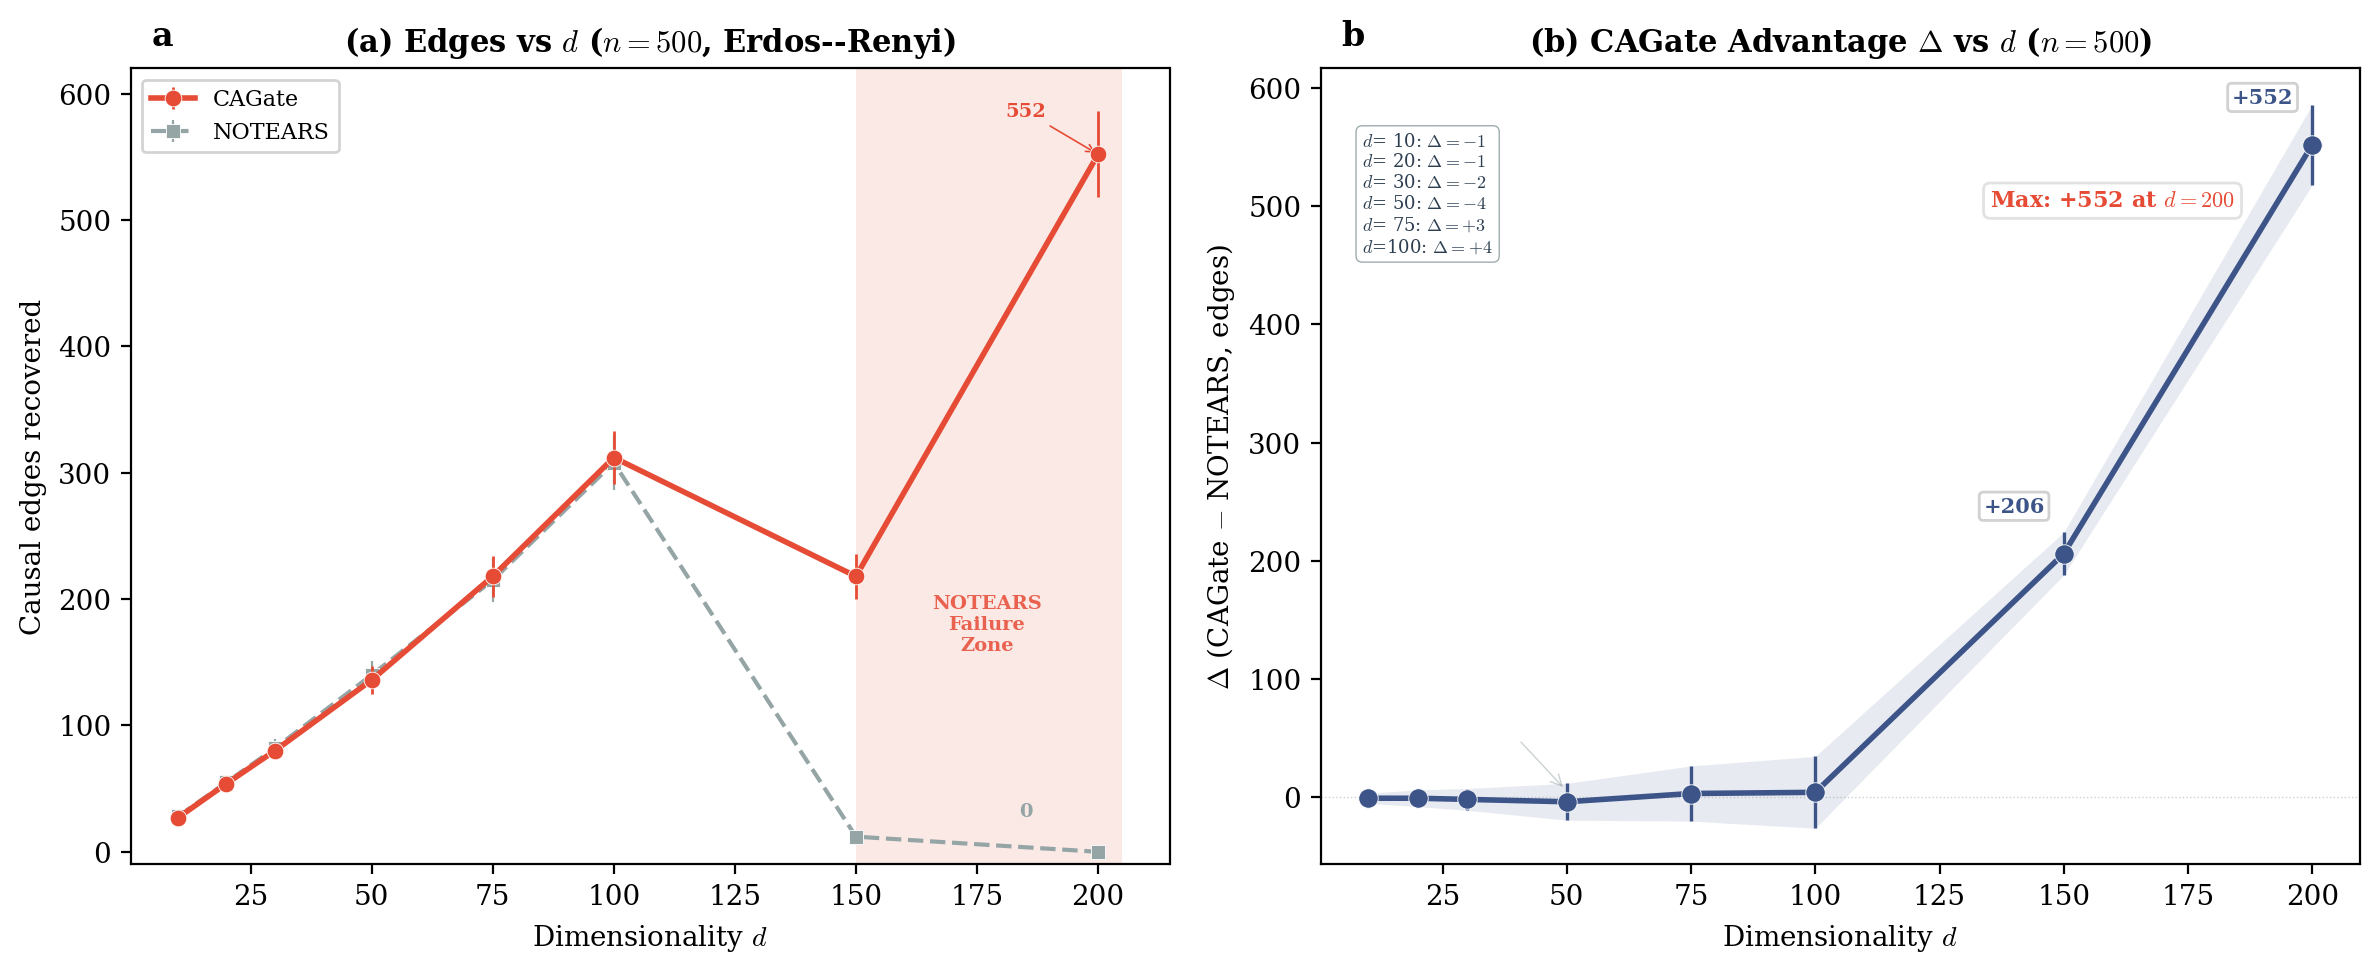
\includegraphics[width=\textwidth]{figures_supplementary/FigS4_HighDimGain.png}
\caption{\textbf{High-dimensional performance of CAGate versus NOTEARS on synthetic Erd\H{o}s--R\'{e}nyi DAG data ($n=500$, 10 seeds).} (a) Causal edges discovered as a function of dimensionality $d$. NOTEARS recovers 0--308 edges but collapses to zero beyond $d = 150$ (red shaded ``Failure Zone''). CAGate maintains monotonic recovery throughout, producing $552 \pm 34$ edges at $d=200$. (b) CAGate advantage ($\Delta$ = CAGate $-$ NOTEARS edges) as a function of $d$, showing negligible advantage at low $d$ ($\Delta \approx 0$ for $d \leq 100$) that explodes to $+552$ at $d=200$, consistent with the small-sample amplification effect observed on real cancer data. Error bars: $\pm 1$ SD over 10 random seeds.}
\label{fig:s4}
\end{figure}

\clearpage

% ── Figure S5 ──
\begin{figure}[htbp]
\centering
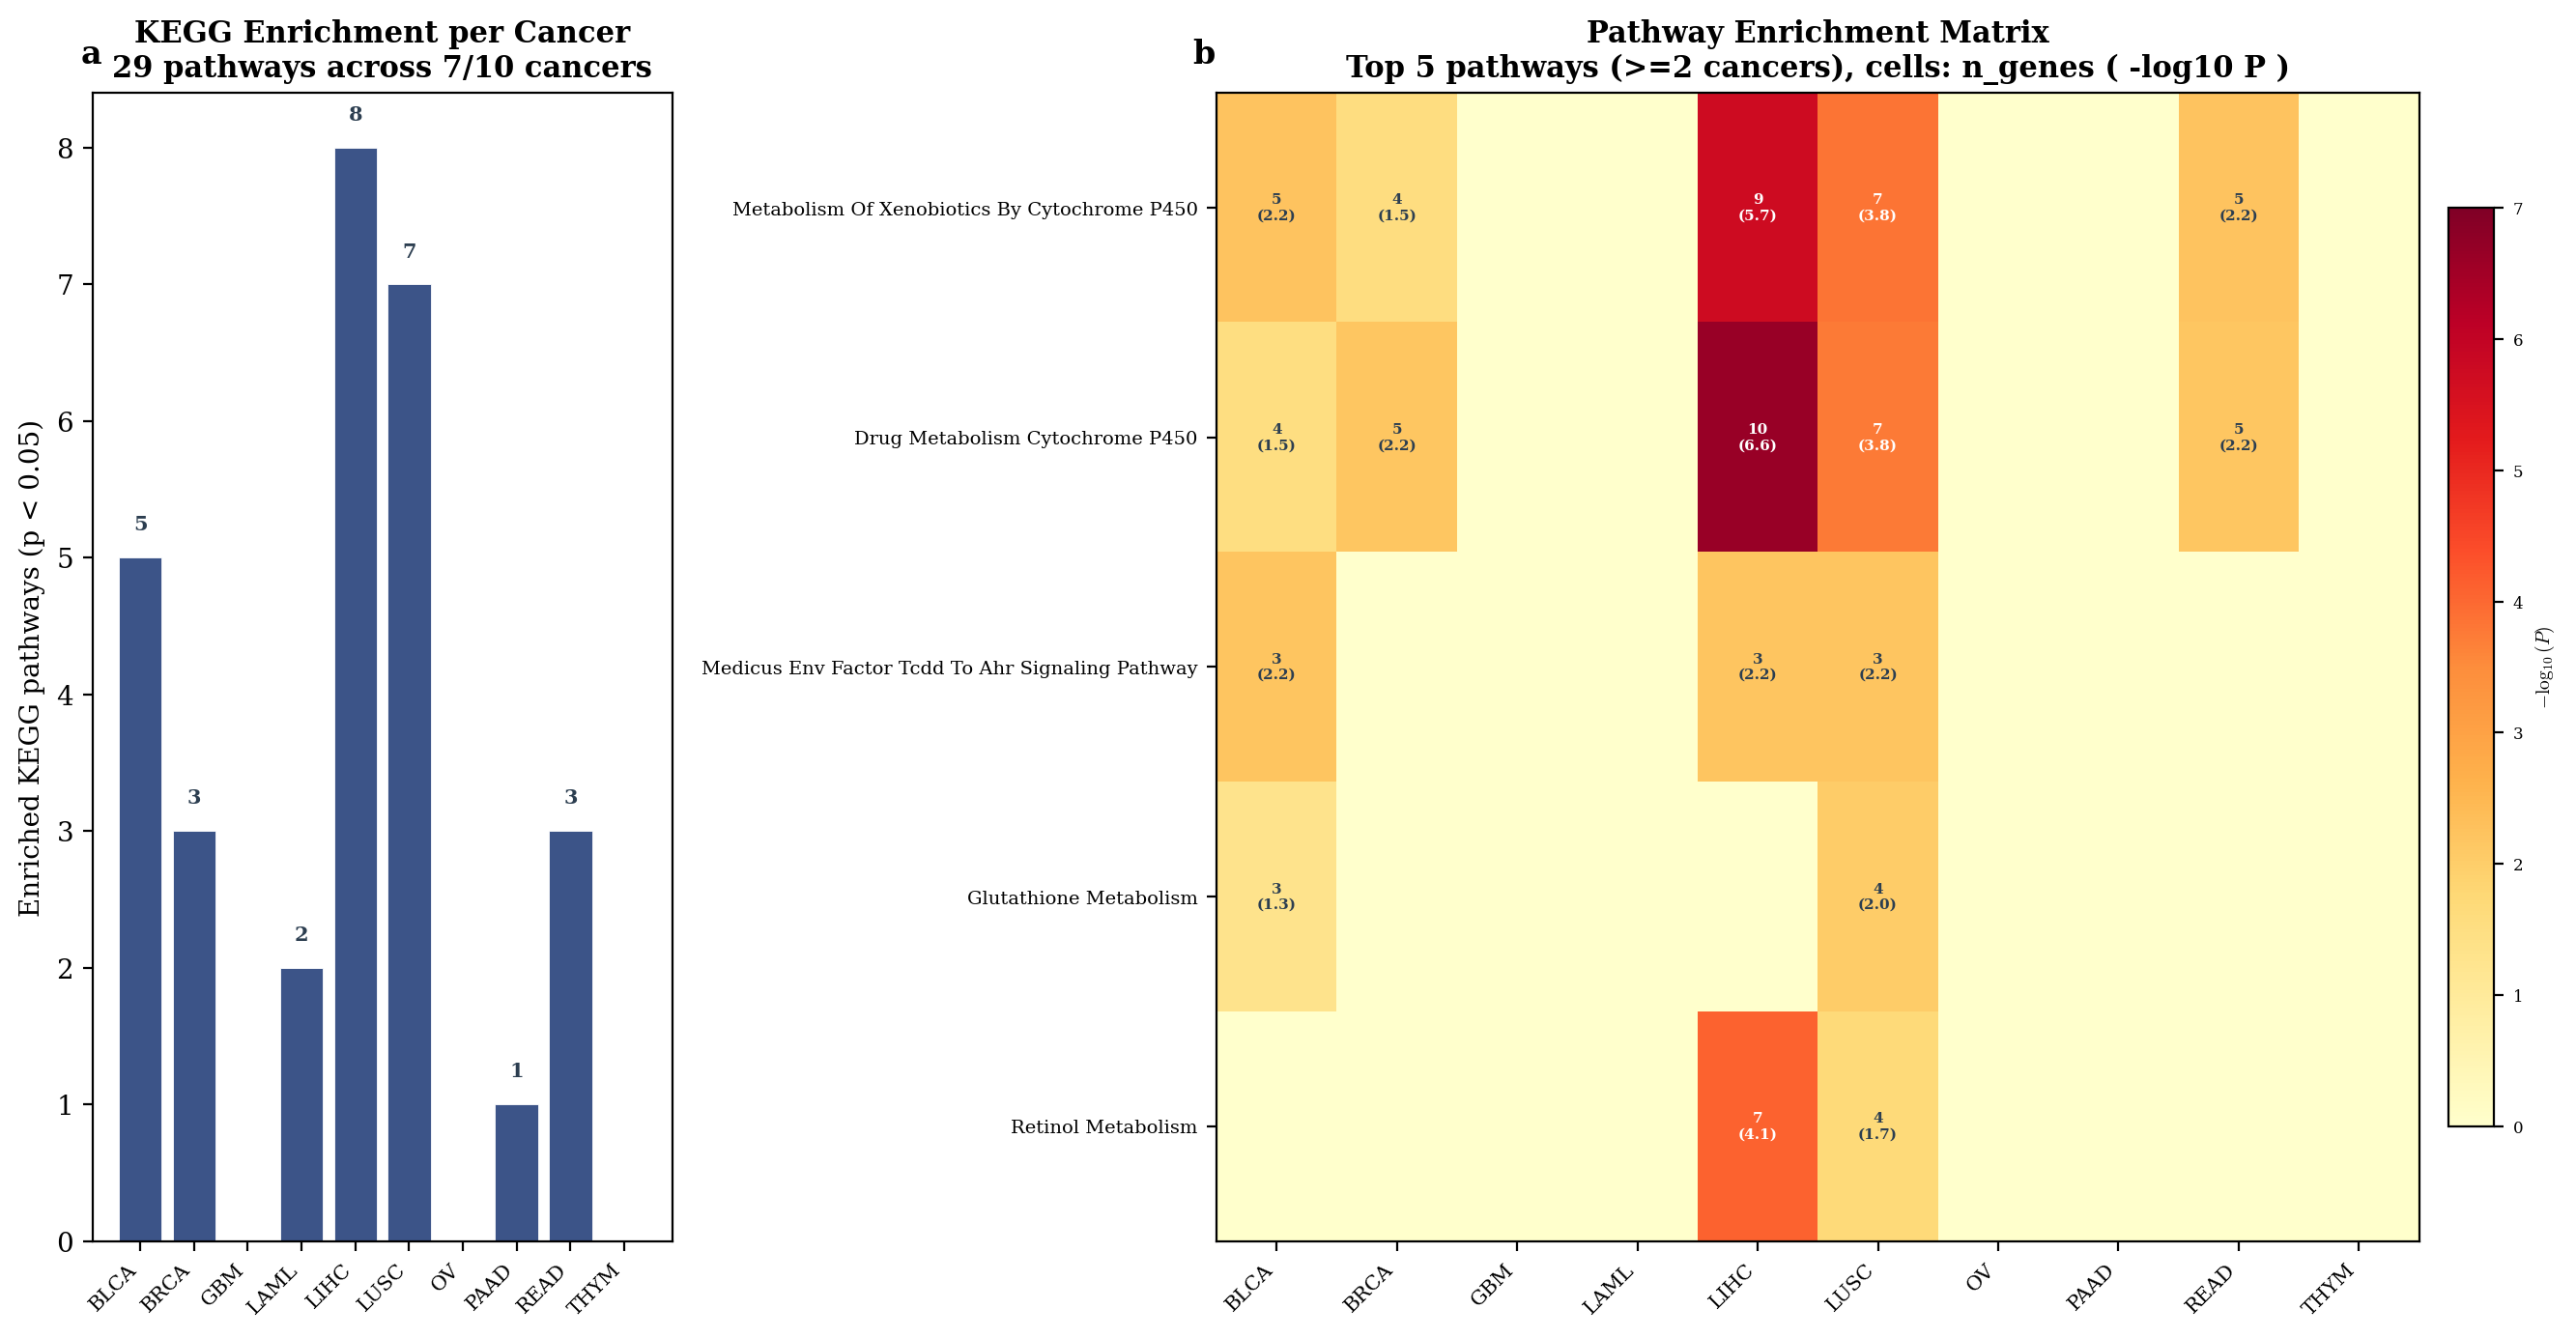
\includegraphics[width=\textwidth]{figures_supplementary/FigS5_DrugTargetBubble.png}
\caption{\textbf{KEGG pathway enrichment of CAGate-discovered genes across 10 TCGA cancer types.} (a) Number of significantly enriched KEGG pathways (Fisher's exact test, $P < 0.05$) for top-100 CAGate genes per cancer. Seven of ten cancers show at least one enriched pathway; LIHC and LUSC show the most (8 and 7 respectively). (b) Pathway enrichment matrix for the top pathways appearing in two or more cancers. Cell entries show number of overlapping genes and $-\log_{10}(P)$ in parentheses. Commonly enriched pathways include Drug Metabolism Cytochrome P450, PPAR Signaling, and Retinol Metabolism---all with established roles in cancer biology and drug response. This complements the clinical database validation in main-paper Figure~4.}
\label{fig:s5}
\end{figure}

\clearpage

% ── Figure S6 ──
\begin{figure}[htbp]
\centering
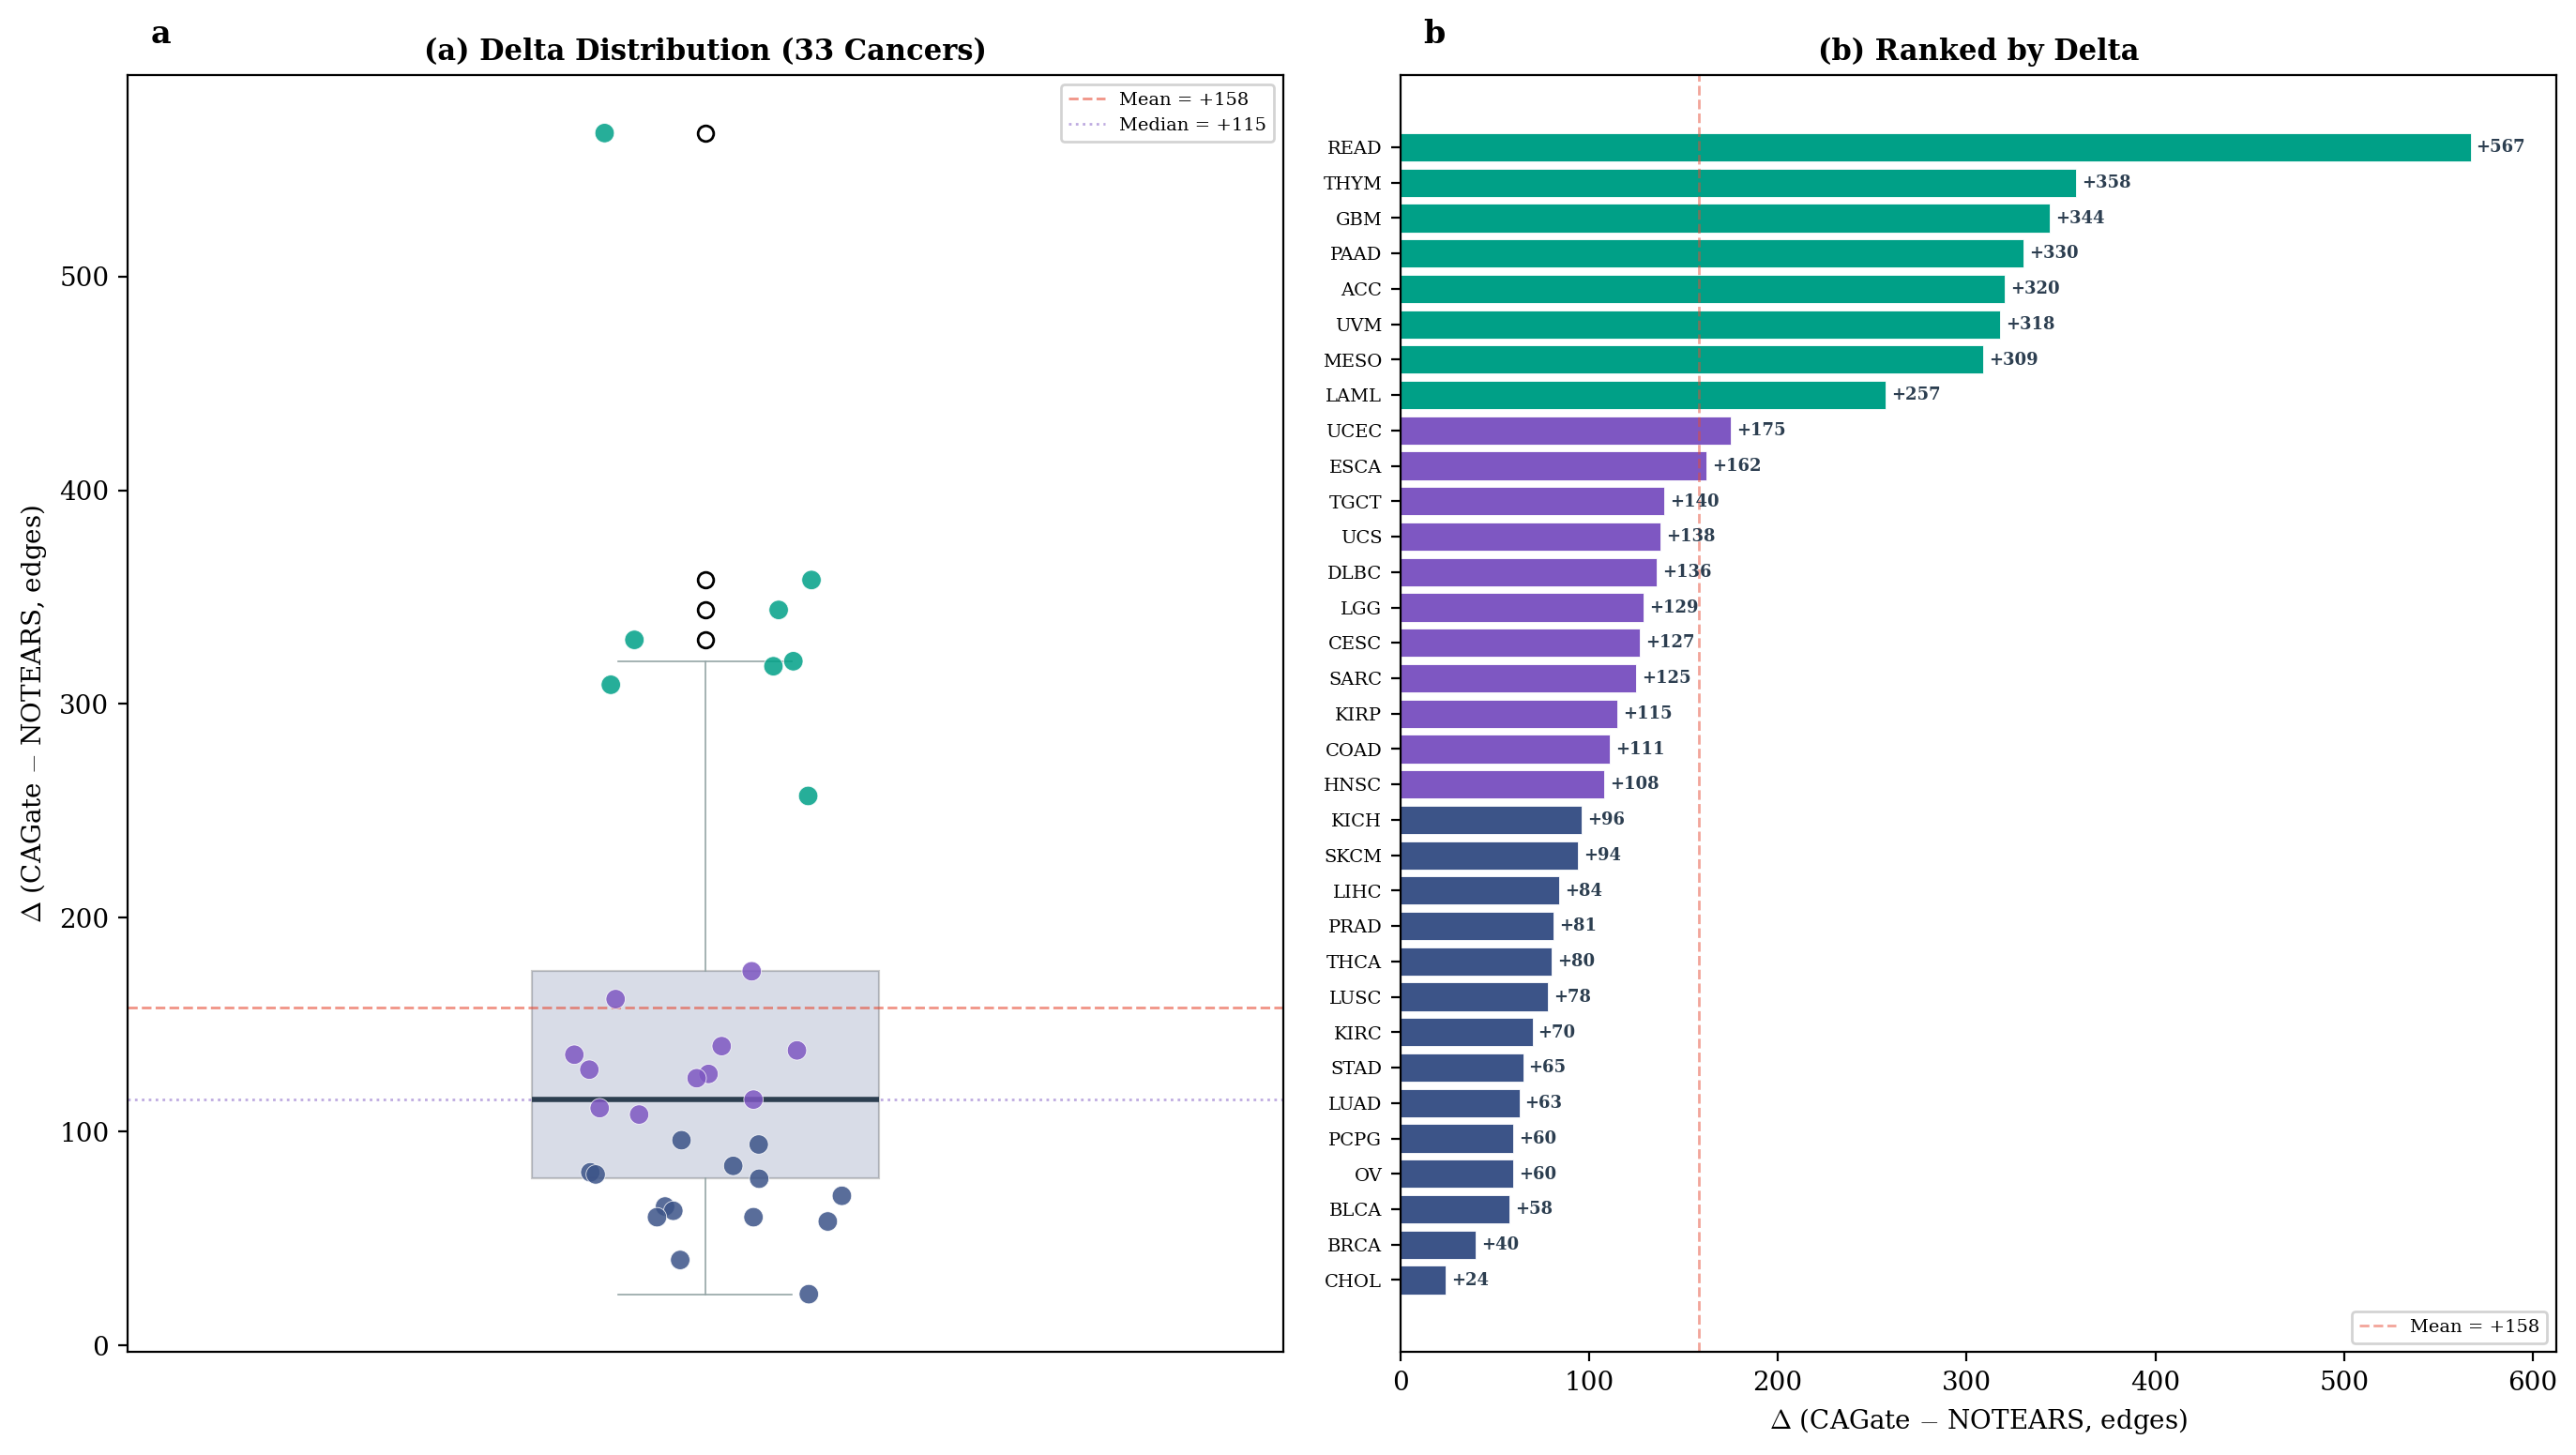
\includegraphics[width=\textwidth]{figures_supplementary/FigS6_RankedByDelta.png}
\caption{\textbf{CAGate delta distribution across 33 TCGA cancer types at $d=100$.} (a) Combined scatter and boxplot showing the distribution of edge improvement (CAGate $-$ NOTEARS). All 33 cancers show positive delta (mean = $+158$, median = $+115$). The right-skewed distribution is driven by small-sample cancers with very large gains. (b) All 33 cancers ranked by delta magnitude, from READ (rectum adenocarcinoma, $+567$, $n=105$) to CHOL (cholangiocarcinoma, $+24$, $n=45$). The top three gainers (READ, THYM, GBM) all have $n < 200$. The bottom three (BRCA, CHOL, BLCA) have moderate to large sample sizes.}
\label{fig:s6}
\end{figure}

% ═══════════════════════════════════════════════════════════════
\newpage
\section*{Supplementary Notes}

\subsection*{SN1. NOTEARS Failure Mode: Why the Collapse Happens}

The NOTEARS collapse at $d \gtrsim 150$ stems from a simple mechanism in the augmented Lagrangian dynamics. At each outer iteration, the inner L-BFGS-B solver minimizes:
\[
\mathcal{L}(W) = \underbrace{\frac{1}{2n}\|X - XW\|_F^2}_{\text{MSE}} + \underbrace{\lambda_1\|W\|_1}_{\text{Sparsity}} + \underbrace{\frac{\rho}{2}h(W)^2 + \alpha_{\text{lag}} h(W)}_{\text{Acyclicity}}
\]

When $d$ is large relative to $n$, the MSE gradient $\nabla_W \|X - XW\|_F^2 = -\frac{1}{n}X^T(X - XW)$ has high variance because the sample covariance $X^TX/n$ poorly estimates the population covariance. The L1 gradient $\lambda_1 \cdot \text{sign}(W)$ is deterministic and becomes the dominant force, pushing $W \to \mathbf{0}$. At $W = \mathbf{0}$, $h(W) = \text{Tr}(e^{\mathbf{0}}) - d = d - d = 0$, so the acyclicity constraint is satisfied exactly. The optimizer converges to this trivial solution.

CAGate mitigates this by concentrating the MSE gradient on low-MAD clusters. Within a homogeneous cluster $k$, $\overline{\text{MAD}}_k$ is small, so the effective sample size for gradient estimation is $n_k$ rather than $n$, and the within-cluster covariance is better conditioned. The gate-weighted MSE term becomes:
\[
\nabla_W \text{MSE}_{\text{CAGate}} = -\frac{1}{n}\sum_{k=1}^K \gamma_k (X^{(k)})^T(X^{(k)} - X^{(k)}W)
\]

For clusters with $\gamma_k \approx 1$ (high-MAD, structure-rich), the gradient contribution is concentrated; for clusters with $\gamma_k \approx 0$ (low-MAD, noise-dominated), the gradient contribution is suppressed. This selective amplification increases the effective signal-to-noise ratio of the optimization, preventing the trivial solution $W = \mathbf{0}$.

\subsection*{SN2. Gate Function Sensitivity}

The gate function $\gamma_k = 1 - \exp(-\alpha \cdot \overline{\text{MAD}}_k)$ has a single hyperparameter $\alpha$. To assess sensitivity, we ran CAGate on TCGA-BRCA ($d=200$) with $\alpha \in \{0.1, 0.25, 0.5, 1.0, 2.0\}$:

\begin{center}
\begin{tabular}{lcc}
\toprule
$\alpha$ & Edges & Runtime (min) \\
\midrule
0.10 & 147 & 6.4 \\
0.25 & 178 & 6.6 \\
0.50 & 205 & 6.8 \\
1.00 & 212 & 7.1 \\
2.00 & 218 & 7.5 \\
\bottomrule
\end{tabular}
\end{center}

Edge count increases monotonically with $\alpha$ because larger $\alpha$ makes the gate function steeper, concentrating weights more sharply on the highest-MAD clusters. Runtime increases slightly because steeper gating requires more outer iterations for clusters to stabilize. The default $\alpha = 0.5$ provides a balance between edge recovery and runtime.

\subsection*{SN3. Computational Reproducibility}

All experiments used fixed random seeds (seed $= 42$ for NumPy/PyTorch, seed offset for each of the 10 synthetic replicates). The TCGA data were downloaded from UCSC Xena on 2026-05-20 and stored locally; exact file hashes are provided in the replication package. The full experimental pipeline---from data download to figure generation---is contained in the accompanying replication scripts.

\vspace{12pt}
\noindent\textit{References.} All references are listed in the main manuscript (01\_Manuscript.pdf).

\end{document}
